\documentclass[12pt,journal,compsoc]{IEEEtran}
% The Computer Society requires 12pt.
% If IEEEtran.cls has not been installed into the LaTeX system files,
% manually specify the path to it like:
% \documentclass[10pt,journal,compsoc]{../sty/IEEEtran}


% For Computer Society journals, IEEEtran defaults to the use of 
% Palatino/Palladio as is done in IEEE Computer Society journals.
% To go back to Times Roman, you can use this code:
%\renewcommand{\rmdefault}{ptm}\selectfont





% Some very useful LaTeX packages include:
% (uncomment the ones you want to load)



% *** MISC UTILITY PACKAGES ***
%
%\usepackage{ifpdf}
% Heiko Oberdiek's ifpdf.sty is very useful if you need conditional
% compilation based on whether the output is pdf or dvi.
% usage:
% \ifpdf
%   % pdf code
% \else
%   % dvi code
% \fi
% The latest version of ifpdf.sty can be obtained from:
% http://www.ctan.org/tex-archive/macros/latex/contrib/oberdiek/
% Also, note that IEEEtran.cls V1.7 and later provides a builtin
% \ifCLASSINFOpdf conditional that works the same way.
% When switching from latex to pdflatex and vice-versa, the compiler may
% have to be run twice to clear warning/error messages.






% *** CITATION PACKAGES ***
%
\ifCLASSOPTIONcompsoc
  % IEEE Computer Society needs nocompress option
  % requires cite.sty v4.0 or later (November 2003)
  \usepackage[nocompress]{cite}
\else
  % normal IEEE
  \usepackage{cite}
\fi
% cite.sty was written by Donald Arseneau
% V1.6 and later of IEEEtran pre-defines the format of the cite.sty package
% \cite{} output to follow that of IEEE. Loading the cite package will
% result in citation numbers being automatically sorted and properly
% "compressed/ranged". e.g., [1], [9], [2], [7], [5], [6] without using
% cite.sty will become [1], [2], [5]--[7], [9] using cite.sty. cite.sty's
% \cite will automatically add leading space, if needed. Use cite.sty's
% noadjust option (cite.sty V3.8 and later) if you want to turn this off
% such as if a citation ever needs to be enclosed in parenthesis.
% cite.sty is already installed on most LaTeX systems. Be sure and use
% version 4.0 (2003-05-27) and later if using hyperref.sty. cite.sty does
% not currently provide for hyperlinked citations.
% The latest version can be obtained at:
% http://www.ctan.org/tex-archive/macros/latex/contrib/cite/
% The documentation is contained in the cite.sty file itself.
%
% Note that some packages require special options to format as the Computer
% Society requires. In particular, Computer Society  papers do not use
% compressed citation ranges as is done in typical IEEE papers
% (e.g., [1]-[4]). Instead, they list every citation separately in order
% (e.g., [1], [2], [3], [4]). To get the latter we need to load the cite
% package with the nocompress option which is supported by cite.sty v4.0
% and later.
%
% Note also the use of a CLASSOPTION conditional provided by 
% IEEEtran.cls V1.7 and later.





% *** GRAPHICS RELATED PACKAGES ***
%
\usepackage[pdftex]{graphicx}
% declare the path(s) where your graphic files are
\graphicspath{{../pdf/}{../jpeg/}}
% and their extensions so you won't have to specify these with
% every instance of \includegraphics
\DeclareGraphicsExtensions{.pdf,.jpeg,.png}



% *** MATH PACKAGES ***
%
%\usepackage[cmex10]{amsmath}
% A popular package from the American Mathematical Society that provides
% many useful and powerful commands for dealing with mathematics. If using
% it, be sure to load this package with the cmex10 option to ensure that
% only type 1 fonts will utilized at all point sizes. Without this option,
% it is possible that some math symbols, particularly those within
% footnotes, will be rendered in bitmap form which will result in a
% document that can not be IEEE Xplore compliant!
%
% Also, note that the amsmath package sets \interdisplaylinepenalty to 10000
% thus preventing page breaks from occurring within multiline equations. Use:
%\interdisplaylinepenalty=2500
% after loading amsmath to restore such page breaks as IEEEtran.cls normally
% does. amsmath.sty is already installed on most LaTeX systems. The latest
% version and documentation can be obtained at:
% http://www.ctan.org/tex-archive/macros/latex/required/amslatex/math/





% *** SPECIALIZED LIST PACKAGES ***
%\usepackage{acronym}
% acronym.sty was written by Tobias Oetiker. This package provides tools for
% managing documents with large numbers of acronyms. (You don't *have* to
% use this package - unless you have a lot of acronyms, you may feel that
% such package management of them is bit of an overkill.)
% Do note that the acronym environment (which lists acronyms) will have a
% problem when used under IEEEtran.cls because acronym.sty relies on the
% description list environment - which IEEEtran.cls has customized for
% producing IEEE style lists. A workaround is to declared the longest
% label width via the IEEEtran.cls \IEEEiedlistdecl global control:
%
% \renewcommand{\IEEEiedlistdecl}{\IEEEsetlabelwidth{SONET}}
% \begin{acronym}
%
% \end{acronym}
% \renewcommand{\IEEEiedlistdecl}{\relax}% remember to reset \IEEEiedlistdecl
%
% instead of using the acronym environment's optional argument.
% The latest version and documentation can be obtained at:
% http://www.ctan.org/tex-archive/macros/latex/contrib/acronym/


%\usepackage{algorithmic}
% algorithmic.sty was written by Peter Williams and Rogerio Brito.
% This package provides an algorithmic environment fo describing algorithms.
% You can use the algorithmic environment in-text or within a figure
% environment to provide for a floating algorithm. Do NOT use the algorithm
% floating environment provided by algorithm.sty (by the same authors) or
% algorithm2e.sty (by Christophe Fiorio) as IEEE does not use dedicated
% algorithm float types and packages that provide these will not provide
% correct IEEE style captions. The latest version and documentation of
% algorithmic.sty can be obtained at:
% http://www.ctan.org/tex-archive/macros/latex/contrib/algorithms/
% There is also a support site at:
% http://algorithms.berlios.de/index.html
% Also of interest may be the (relatively newer and more customizable)
% algorithmicx.sty package by Szasz Janos:
% http://www.ctan.org/tex-archive/macros/latex/contrib/algorithmicx/




% *** ALIGNMENT PACKAGES ***
%
%\usepackage{array}
% Frank Mittelbach's and David Carlisle's array.sty patches and improves
% the standard LaTeX2e array and tabular environments to provide better
% appearance and additional user controls. As the default LaTeX2e table
% generation code is lacking to the point of almost being broken with
% respect to the quality of the end results, all users are strongly
% advised to use an enhanced (at the very least that provided by array.sty)
% set of table tools. array.sty is already installed on most systems. The
% latest version and documentation can be obtained at:
% http://www.ctan.org/tex-archive/macros/latex/required/tools/


%\usepackage{mdwmath}
%\usepackage{mdwtab}
% Also highly recommended is Mark Wooding's extremely powerful MDW tools,
% especially mdwmath.sty and mdwtab.sty which are used to format equations
% and tables, respectively. The MDWtools set is already installed on most
% LaTeX systems. The lastest version and documentation is available at:
% http://www.ctan.org/tex-archive/macros/latex/contrib/mdwtools/


% IEEEtran contains the IEEEeqnarray family of commands that can be used to
% generate multiline equations as well as matrices, tables, etc., of high
% quality.


%\usepackage{eqparbox}
% Also of notable interest is Scott Pakin's eqparbox package for creating
% (automatically sized) equal width boxes - aka "natural width parboxes".
% Available at:
% http://www.ctan.org/tex-archive/macros/latex/contrib/eqparbox/




% *** SUBFIGURE PACKAGES ***
%\ifCLASSOPTIONcompsoc
%  \usepackage[caption=false,font=normalsize,labelfont=sf,textfont=sf]{subfig}
%\else
%  \usepackage[caption=false,font=footnotesize]{subfig}
%\fi
% subfig.sty, written by Steven Douglas Cochran, is the modern replacement
% for subfigure.sty, the latter of which is no longer maintained and is
% incompatible with some LaTeX packages including fixltx2e. However,
% subfig.sty requires and automatically loads Axel Sommerfeldt's caption.sty
% which will override IEEEtran.cls' handling of captions and this will result
% in non-IEEE style figure/table captions. To prevent this problem, be sure
% and invoke subfig.sty's "caption=false" package option (available since
% subfig.sty version 1.3, 2005/06/28) as this is will preserve IEEEtran.cls
% handling of captions.
% Note that the Computer Society format requires a larger sans serif font
% than the serif footnote size font used in traditional IEEE formatting
% and thus the need to invoke different subfig.sty package options depending
% on whether compsoc mode has been enabled.
%
% The latest version and documentation of subfig.sty can be obtained at:
% http://www.ctan.org/tex-archive/macros/latex/contrib/subfig/




% *** FLOAT PACKAGES ***
%
\usepackage{fixltx2e}
% fixltx2e, the successor to the earlier fix2col.sty, was written by
% Frank Mittelbach and David Carlisle. This package corrects a few problems
% in the LaTeX2e kernel, the most notable of which is that in current
% LaTeX2e releases, the ordering of single and double column floats is not
% guaranteed to be preserved. Thus, an unpatched LaTeX2e can allow a
% single column figure to be placed prior to an earlier double column
% figure. The latest version and documentation can be found at:
% http://www.ctan.org/tex-archive/macros/latex/base/


%\usepackage{stfloats}
% stfloats.sty was written by Sigitas Tolusis. This package gives LaTeX2e
% the ability to do double column floats at the bottom of the page as well
% as the top. (e.g., "\begin{figure*}[!b]" is not normally possible in
% LaTeX2e). It also provides a command:
%\fnbelowfloat
% to enable the placement of footnotes below bottom floats (the standard
% LaTeX2e kernel puts them above bottom floats). This is an invasive package
% which rewrites many portions of the LaTeX2e float routines. It may not work
% with other packages that modify the LaTeX2e float routines. The latest
% version and documentation can be obtained at:
% http://www.ctan.org/tex-archive/macros/latex/contrib/sttools/
% Do not use the stfloats baselinefloat ability as IEEE does not allow
% \baselineskip to stretch. Authors submitting work to the IEEE should note
% that IEEE rarely uses double column equations and that authors should try
% to avoid such use. Do not be tempted to use the cuted.sty or midfloat.sty
% packages (also by Sigitas Tolusis) as IEEE does not format its papers in
% such ways.
% Do not attempt to use stfloats with fixltx2e as they are incompatible.
% Instead, use Morten Hogholm'a dblfloatfix which combines the features
% of both fixltx2e and stfloats:
%
\usepackage{dblfloatfix}
% The latest version can be found at:
% http://www.ctan.org/tex-archive/macros/latex/contrib/dblfloatfix/


%\ifCLASSOPTIONcaptionsoff
%  \usepackage[nomarkers]{endfloat}
% \let\MYoriglatexcaption\caption
% \renewcommand{\caption}[2][\relax]{\MYoriglatexcaption[#2]{#2}}
%\fi
% endfloat.sty was written by James Darrell McCauley, Jeff Goldberg and 
% Axel Sommerfeldt. This package may be useful when used in conjunction with 
% IEEEtran.cls'  captionsoff option. Some IEEE journals/societies require that
% submissions have lists of figures/tables at the end of the paper and that
% figures/tables without any captions are placed on a page by themselves at
% the end of the document. If needed, the draftcls IEEEtran class option or
% \CLASSINPUTbaselinestretch interface can be used to increase the line
% spacing as well. Be sure and use the nomarkers option of endfloat to
% prevent endfloat from "marking" where the figures would have been placed
% in the text. The two hack lines of code above are a slight modification of
% that suggested by in the endfloat docs (section 8.4.1) to ensure that
% the full captions always appear in the list of figures/tables - even if
% the user used the short optional argument of \caption[]{}.
% IEEE papers do not typically make use of \caption[]'s optional argument,
% so this should not be an issue. A similar trick can be used to disable
% captions of packages such as subfig.sty that lack options to turn off
% the subcaptions:
% For subfig.sty:
% \let\MYorigsubfloat\subfloat
% \renewcommand{\subfloat}[2][\relax]{\MYorigsubfloat[]{#2}}
% However, the above trick will not work if both optional arguments of
% the \subfloat command are used. Furthermore, there needs to be a
% description of each subfigure *somewhere* and endfloat does not add
% subfigure captions to its list of figures. Thus, the best approach is to
% avoid the use of subfigure captions (many IEEE journals avoid them anyway)
% and instead reference/explain all the subfigures within the main caption.
% The latest version of endfloat.sty and its documentation can obtained at:
% http://www.ctan.org/tex-archive/macros/latex/contrib/endfloat/
%
% The IEEEtran \ifCLASSOPTIONcaptionsoff conditional can also be used
% later in the document, say, to conditionally put the References on a 
% page by themselves.





% *** PDF, URL AND HYPERLINK PACKAGES ***
%
\usepackage{url}
% url.sty was written by Donald Arseneau. It provides better support for
% handling and breaking URLs. url.sty is already installed on most LaTeX
% systems. The latest version and documentation can be obtained at:
% http://www.ctan.org/tex-archive/macros/latex/contrib/url/
% Basically, \url{my_url_here}.


% NOTE: PDF thumbnail features are not required in IEEE papers
%       and their use requires extra complexity and work.
\ifCLASSINFOpdf
  \usepackage[pdftex]{thumbpdf}
\else
  \usepackage[dvips]{thumbpdf}
\fi
% thumbpdf.sty and its companion Perl utility were written by Heiko Oberdiek.
% It allows the user a way to produce PDF documents that contain fancy
% thumbnail images of each of the pages (which tools like acrobat reader can
% utilize). This is possible even when using dvi->ps->pdf workflow if the
% correct thumbpdf driver options are used. thumbpdf.sty incorporates the
% file containing the PDF thumbnail information (filename.tpm is used with
% dvips, filename.tpt is used with pdftex, where filename is the base name of
% your tex document) into the final ps or pdf output document. An external
% utility, the thumbpdf *Perl script* is needed to make these .tpm or .tpt
% thumbnail files from a .ps or .pdf version of the document (which obviously
% does not yet contain pdf thumbnails). Thus, one does a:
% 
% thumbpdf filename.pdf 
%
% to make a filename.tpt, and:
%
% thumbpdf --mode dvips filename.ps
%
% to make a filename.tpm which will then be loaded into the document by
% thumbpdf.sty the NEXT time the document is compiled (by pdflatex or
% latex->dvips->ps2pdf). Users must be careful to regenerate the .tpt and/or
% .tpm files if the main document changes and then to recompile the
% document to incorporate the revised thumbnails to ensure that thumbnails
% match the actual pages. It is easy to forget to do this!
% 
% Unix systems come with a Perl interpreter. However, MS Windows users
% will usually have to install a Perl interpreter so that the thumbpdf
% script can be run. The Ghostscript PS/PDF interpreter is also required.
% See the thumbpdf docs for details. The latest version and documentation
% can be obtained at.
% http://www.ctan.org/tex-archive/support/thumbpdf/


% NOTE: PDF hyperlink and bookmark features are not required in IEEE
%       papers and their use requires extra complexity and work.
% *** IF USING HYPERREF BE SURE AND CHANGE THE EXAMPLE PDF ***
% *** TITLE/SUBJECT/AUTHOR/KEYWORDS INFO BELOW!!           ***
\ifCLASSOPTIONpeerreview
\newcommand\MYhyperrefoptions{bookmarks=true,bookmarksnumbered=true,
	pdfpagemode={UseOutlines},plainpages=false,pdfpagelabels=true,
	colorlinks=true,linkcolor={black},citecolor={black},urlcolor={black},
	pdftitle={Requrirements to send unobservable messages accross the internet},%<!CHANGE!
	pdfsubject={Unobservable Messages},%<!CHANGE!
	pdfkeywords={messages, unobservable}}%<^!CHANGE!
\else
\newcommand\MYhyperrefoptions{bookmarks=true,bookmarksnumbered=true,
pdfpagemode={UseOutlines},plainpages=false,pdfpagelabels=true,
colorlinks=true,linkcolor={black},citecolor={black},urlcolor={black},
pdftitle={Requrirements to send unobservable messages accross the internet},%<!CHANGE!
pdfsubject={Unobservable Messages},%<!CHANGE!
pdfauthor={Martin Gwerder},%<!CHANGE!
pdfkeywords={messages, unobservable}}%<^!CHANGE!
\fi
%\ifCLASSINFOpdf
\usepackage[\MYhyperrefoptions,pdftex]{hyperref}
%\else
%\usepackage[\MYhyperrefoptions,breaklinks=true,dvips]{hyperref}
%\usepackage{breakurl}
%\fi
% One significant drawback of using hyperref under DVI output is that the
% LaTeX compiler cannot break URLs across lines or pages as can be done
% under pdfLaTeX's PDF output via the hyperref pdftex driver. This is
% probably the single most important capability distinction between the
% DVI and PDF output. Perhaps surprisingly, all the other PDF features
% (PDF bookmarks, thumbnails, etc.) can be preserved in
% .tex->.dvi->.ps->.pdf workflow if the respective packages/scripts are
% loaded/invoked with the correct driver options (dvips, etc.). 
% As most IEEE papers use URLs sparingly (mainly in the references), this
% may not be as big an issue as with other publications.
%
% That said, Vilar Camara Neto created his breakurl.sty package which
% permits hyperref to easily break URLs even in dvi mode.
% Note that breakurl, unlike most other packages, must be loaded
% AFTER hyperref. The latest version of breakurl and its documentation can
% be obtained at:
% http://www.ctan.org/tex-archive/macros/latex/contrib/breakurl/
% breakurl.sty is not for use under pdflatex pdf mode.
%
% The advanced features offer by hyperref.sty are not required for IEEE
% submission, so users should weigh these features against the added
% complexity of use.
% The package options above demonstrate how to enable PDF bookmarks
% (a type of table of contents viewable in Acrobat Reader) as well as
% PDF document information (title, subject, author and keywords) that is
% viewable in Acrobat reader's Document_Properties menu. PDF document
% information is also used extensively to automate the cataloging of PDF
% documents. The above set of options ensures that hyperlinks will not be
% colored in the text and thus will not be visible in the printed page,
% but will be active on "mouse over". USING COLORS OR OTHER HIGHLIGHTING
% OF HYPERLINKS CAN RESULT IN DOCUMENT REJECTION BY THE IEEE, especially if
% these appear on the "printed" page. IF IN DOUBT, ASK THE RELEVANT
% SUBMISSION EDITOR. You may need to add the option hypertexnames=false if
% you used duplicate equation numbers, etc., but this should not be needed
% in normal IEEE work.
% The latest version of hyperref and its documentation can be obtained at:
% http://www.ctan.org/tex-archive/macros/latex/contrib/hyperref/





% *** Do not adjust lengths that control margins, column widths, etc. ***
% *** Do not use packages that alter fonts (such as pslatex).         ***
% There should be no need to do such things with IEEEtran.cls V1.6 and later.
% (Unless specifically asked to do so by the journal or conference you plan
% to submit to, of course. )


% correct bad hyphenation here
\hyphenation{op-tical net-works semi-conduc-tor}

\usepackage{zref-user}

\begin{document}
%
% paper title
% can use linebreaks \\ within to get better formatting as desired
% Do not put math or special symbols in the title.
\title{Requirements to send unobservable messages accross the internet}
%
%
% author names and IEEE memberships
% note positions of commas and nonbreaking spaces ( ~ ) LaTeX will not break
% a structure at a ~ so this keeps an author's name from being broken across
% two lines.
% use \thanks{} to gain access to the first footnote area
% a separate \thanks must be used for each paragraph as LaTeX2e's \thanks
% was not built to handle multiple paragraphs
%
%
%\IEEEcompsocitemizethanks is a special \thanks that produces the bulleted
% lists the Computer Society journals use for "first footnote" author
% affiliations. Use \IEEEcompsocthanksitem which works much like \item
% for each affiliation group. When not in compsoc mode,
% \IEEEcompsocitemizethanks becomes like \thanks and
% \IEEEcompsocthanksitem becomes a line break with idention. This
% facilitates dual compilation, although admittedly the differences in the
% desired content of \author between the different types of papers makes a
% one-size-fits-all approach a daunting prospect. For instance, compsoc 
% journal papers have the author affiliations above the "Manuscript
% received ..."  text while in non-compsoc journals this is reversed. Sigh.

\ifCLASSOPTIONpeerreview
\author{}
\else
\author{Martin Gwerder% <-this % stops a space
%\IEEEcompsocitemizethanks{\IEEEcompsocthanksitem none?.\protect\\
% note need leading \protect in front of \\ to get a newline within \thanks as
% \\ is fragile and will error, could use \hfil\break instead.
%E-mail: m.gwerder@unibas.ch
%\IEEEcompsocthanksitem J. Doe and J. Doe are with Anonymous University.}% <-this % stops a space
%\thanks{Manuscript received April 19, 2005; revised December 27, 2012.}
}
\fi

% note the % following the last \IEEEmembership and also \thanks - 
% these prevent an unwanted space from occurring between the last author name
% and the end of the author line. i.e., if you had this:
% 
% \author{....lastname \thanks{...} \thanks{...} }
%                     ^------------^------------^----Do not want these spaces!
%
% a space would be appended to the last name and could cause every name on that
% line to be shifted left slightly. This is one of those "LaTeX things". For
% instance, "\textbf{A} \textbf{B}" will typeset as "A B" not "AB". To get
% "AB" then you have to do: "\textbf{A}\textbf{B}"
% \thanks is no different in this regard, so shield the last } of each \thanks
% that ends a line with a % and do not let a space in before the next \thanks.
% Spaces after \IEEEmembership other than the last one are OK (and needed) as
% you are supposed to have spaces between the names. For what it is worth,
% this is a minor point as most people would not even notice if the said evil
% space somehow managed to creep in.

% The paper headers
\ifCLASSOPTIONpeerreview
\markboth{}{Requirements to send unobservable messages across the internet}
\else
\markboth{Security \& Privacy,~Vol.~??, No.??, Mai~2015}%
{Gwerder: Requirements to send unobservable messages across the internet}
\fi
% The only time the second header will appear is for the odd numbered pages
% after the title page when using the twoside option.
% 
% *** Note that you probably will NOT want to include the author's ***
% *** name in the headers of peer review papers.                   ***
% You can use \ifCLASSOPTIONpeerreview for conditional compilation here if
% you desire.



% The publisher's ID mark at the bottom of the page is less important with
% Computer Society journal papers as those publications place the marks
% outside of the main text columns and, therefore, unlike regular IEEE
% journals, the available text space is not reduced by their presence.
% If you want to put a publisher's ID mark on the page you can do it like
% this:
%\IEEEpubid{0000--0000/00\$00.00~\copyright~2012 IEEE}
% or like this to get the Computer Society new two part style.
%\IEEEpubid{\makebox[\columnwidth]{\hfill 0000--0000/00/\$00.00~\copyright~2012 IEEE}%
%\hspace{\columnsep}\makebox[\columnwidth]{Published by the IEEE Computer Society\hfill}}
% Remember, if you use this you must call \IEEEpubidadjcol in the second
% column for its text to clear the IEEEpubid mark (Computer Society journal
% papers don't need this extra clearance.)



% use for special paper notices
%\IEEEspecialpapernotice{(Invited Paper)}



% for Computer Society papers, we must declare the abstract and index terms
% PRIOR to the title within the \IEEEtitleabstractindextext IEEEtran
% command as these need to go into the title area created by \maketitle.
% As a general rule, do not put math, special symbols or citations
% in the abstract or keywords.
\IEEEtitleabstractindextext{%
\begin{abstract}
In this paper We elaborate all criteria required to create a system capable of transporting messages unobserved through public networks. This is done by collecting all requirements based on the assumed capabilities of the participants. Sending unobservable messages is much harder as generally assumed. It involves a lot of parameters such as "acceptance" or "trust" which are commonly overlooked because of the technical approach most authors prefer. Using a holistic view to the topic we collect all requirements for such a system and categorise them. We furthermore describe why certain systems may not be considered unobservable at any time by definition.
\end{abstract}

% Note that keywords are not normally used for peerreview papers.
\begin{IEEEkeywords}
Data privacy, Message systems, Security
\end{IEEEkeywords}}


% make the title area
\maketitle


% To allow for easy dual compilation without having to reenter the
% abstract/keywords data, the \IEEEtitleabstractindextext text will
% not be used in maketitle, but will appear (i.e., to be "transported")
% here as \IEEEdisplaynontitleabstractindextext when compsoc mode
% is not selected <OR> if conference mode is selected - because compsoc
% conference papers position the abstract like regular (non-compsoc)
% papers do!
\IEEEdisplaynontitleabstractindextext
% \IEEEdisplaynontitleabstractindextext has no effect when using
% compsoc under a non-conference mode.


% For peer review papers, you can put extra information on the cover
% page as needed:
% \ifCLASSOPTIONpeerreview
% \begin{center} \bfseries EDICS Category: 3-BBND \end{center}
% \fi
%
% For peerreview papers, this IEEEtran command inserts a page break and
% creates the second title. It will be ignored for other modes.
\IEEEpeerreviewmaketitle



\section{Introduction}
% Computer Society journal papers do something a tad strange with the very
% first section heading (almost always called "Introduction"). They place it
% ABOVE the main text! IEEEtran.cls currently does not do this for you.
% However, You can achieve this effect by making LaTeX jump through some
% hoops via something like:
%
%\ifCLASSOPTIONcompsoc
%  \noindent\raisebox{2\baselineskip}[0pt][0pt]%
%  {\parbox{\columnwidth}{\section{Introduction}\label{sec:introduction}%
%  \global\everypar=\everypar}}%
%  \vspace{-1\baselineskip}\vspace{-\parskip}\par
%\else
%  \section{Introduction}\label{sec:introduction}\par
%\fi
%
% Admittedly, this is a hack and may well be fragile, but seems to do the
% trick for me. Note the need to keep any \label that may be used right
% after \section in the above as the hack puts \section within a raised box.



% The very first letter is a 2 line initial drop letter followed
% by the rest of the first word in caps (small caps for compsoc).
% 
% form to use if the first word consists of a single letter:
% \IEEEPARstart{A}{demo} file is ....
% 
% form to use if you need the single drop letter followed by
% normal text (unknown if ever used by IEEE):
% \IEEEPARstart{A}{}demo file is ....
% 
% Some journals put the first two words in caps:
% \IEEEPARstart{T}{his demo} file is ....
% 
% Here we have the typical use of a "T" for an initial drop letter
% and "HIS" in caps to complete the first word.
\IEEEPARstart{W}{e} do send messages across the internet every day. Most of them seem to be considered as "not valuable". However -- secret services, advertising companies and researchers have found means to extract data from these messages and create profiles of all participating parties. These profiles often contain very valuable and personal information. The information collected contains often intimate details about all aspects of a person. Even worse: These details might be used against a sender, a recipient or even another peer-partner if they are considered a problem. To give a drastic example: This may happen if someone is a peer-partner to more than one person that is suspected to be a terrorist.\par

As economic aspects are in favour of this kind of data harvesting we can not expect this problem to solve itself. We do need the possibility to send information across public networks which do not disclose personal informations about any of the involved parties. A naive approach would be to encrypt all messages. While this might be sufficient to hide the content of a message it still leaks a lot of information. Even in a perfectly encrypted message the system still needs routing information (such as sender and recipient) to pass on the message. Using this and the technical information we have we may extract many valuable details such as sender, recipient, movement patterns of them, frequency of sending messages between them, average message length, classification of use scheme, preferred services, used devices and clients, and so on.\par
This does not solely apply to personal information. On a similar level it does disclose partnerships between companies, and reveal informations such as research, negotiations, and legal affairs.
\par
There are lots of works\cite{tor-design}\cite{mixmaster-spec}\cite{xor-trees}\cite{Levine:2002}\cite{chaum-mix} that relate to anonymous message transfer. However -- none of these works (with exception to TOR\cite{tor-design}) have been widely adopted in the internet. The reason for this is usually that research tends to concentrate on the method to transport the message and fail at the same time completely to take the real world and its problems into account. 

\begin{figure}
	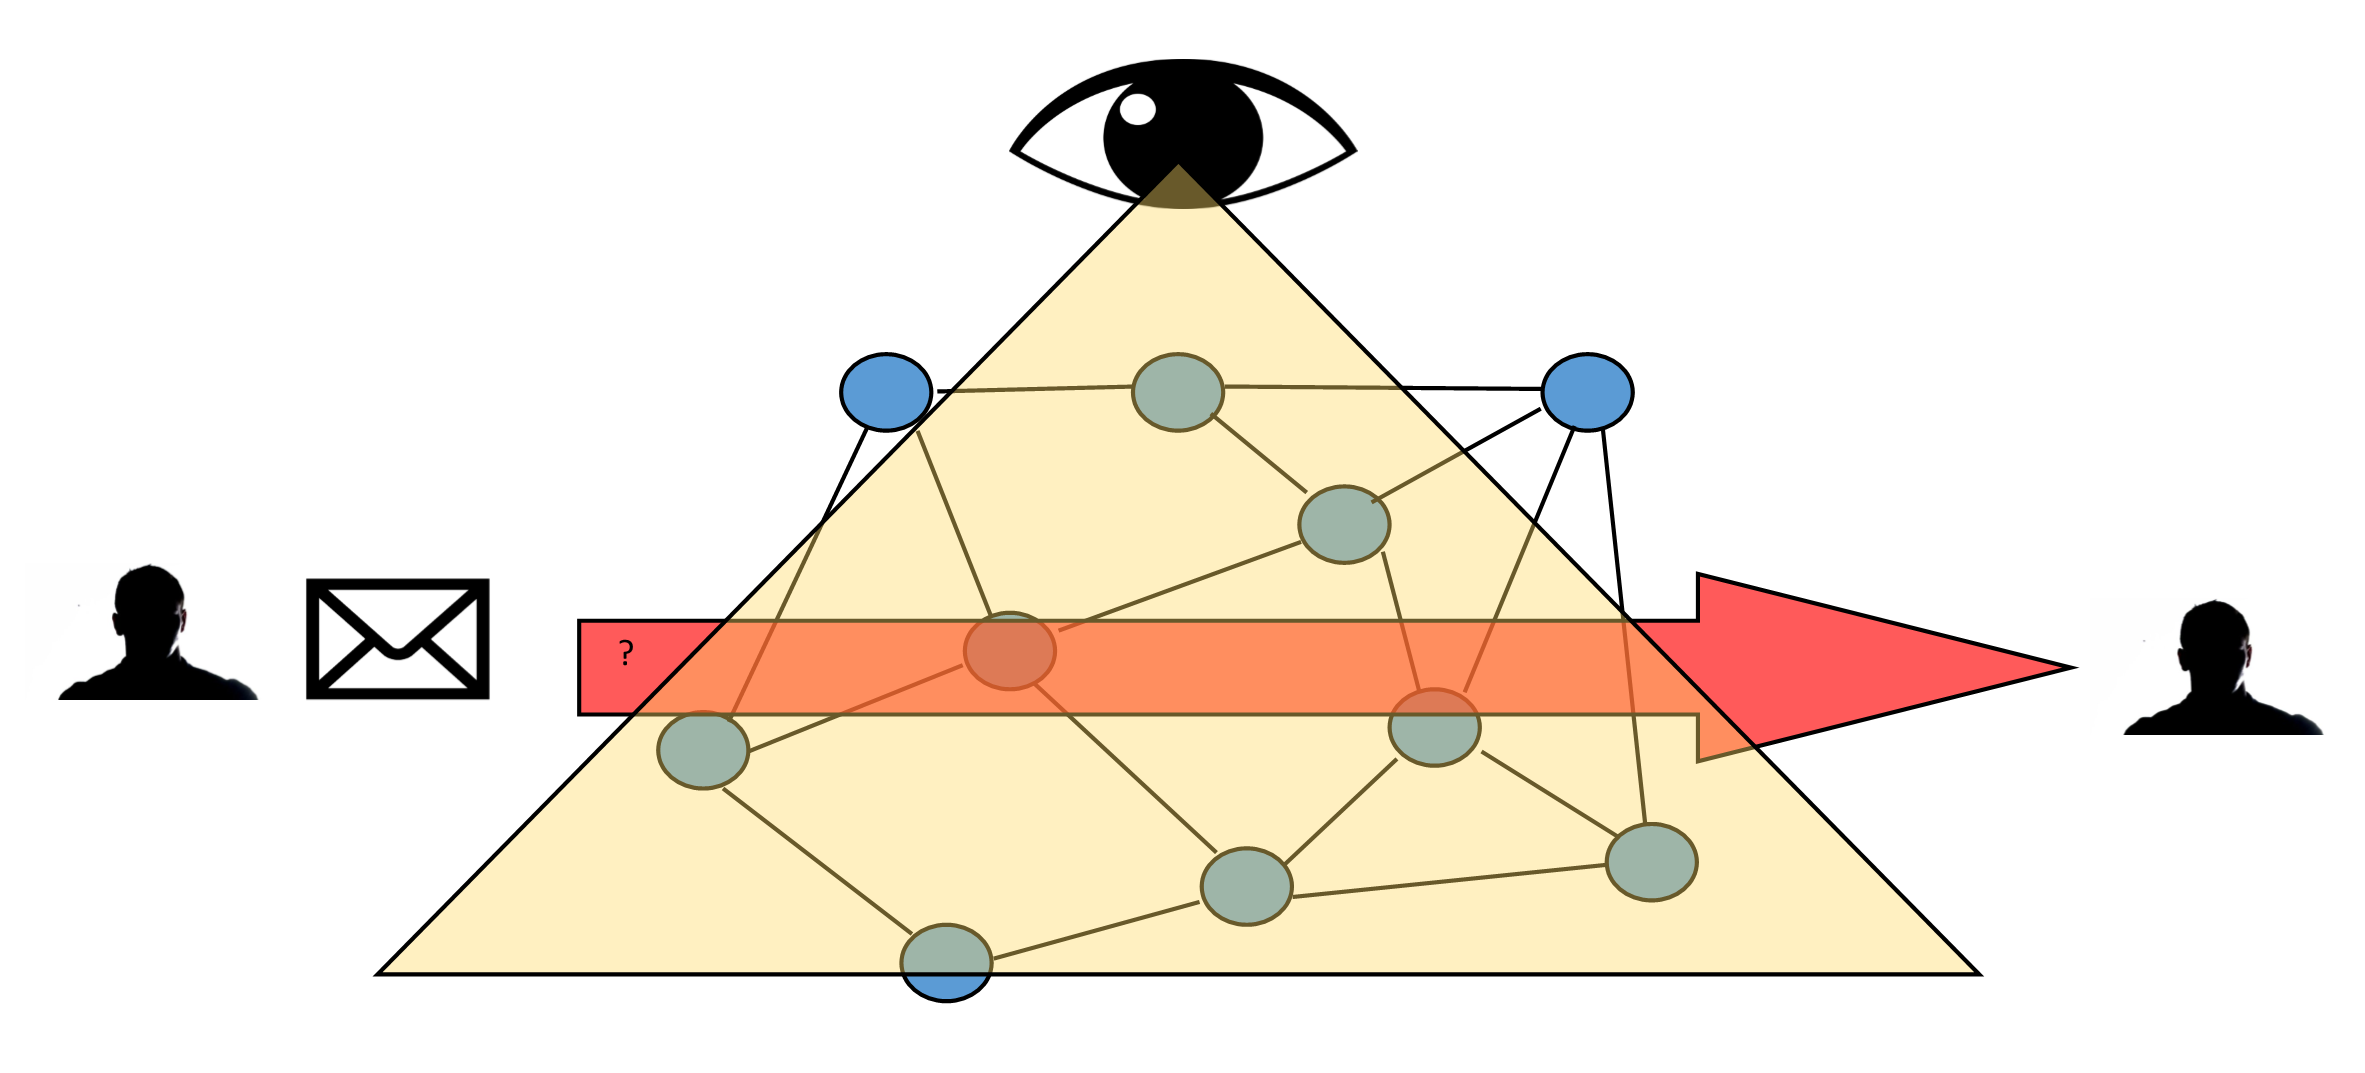
\includegraphics[width=0.9\linewidth]{../poster/messagetransfer.png}
	\caption{sending unobservable messages is not easy}
\end{figure}

In this paper we analyse what is really required to build a service sending unobservable messages. I categorize them and try to build a foundation for future research on this topic.
\par
\ifCLASSOPTIONpeerreview
\else
\hfill gwm
 
\hfill Mai 27, 2015
\fi

\section{Methods}
I assume that we do have a \emph{system} which may or may not require an \emph{infrastructure}. An \emph{infrastructure} may contain one or more participating {nodes}. These \emph{nodes} serve one or more purposes, do have an \emph{owner} that is capable of administering it, and may have \emph{users} that use them. Users are either message \emph{sender} or \emph{recipients}.
\par
On the thread side we do have an \emph{observer} that is capable of monitoring all traffic in the public network and wants to collect data. He may cloak himself as \emph{user} or \emph{owner} and introduce malicious \emph{nodes} into any part of the \emph{system}.
\par
For a more verbose definition see Appendix~\ref{app:definitions}. The \emph{nodes}'s are connected through a packet based network (for ease of argumentation an IP based network is assumed). For definitions of terms such as "unobservable", "anonymity", "psudonymity", "unlinkability" please refer to\cite{pfitzmann2010terminology}.

% needed in second column of first page if using \IEEEpubid
%\IEEEpubidadjcol

\section{Results}
Requirements for an unobservable system may be categorised into three groups:
\begin{itemize}
	\item Acceptance requirements
	\item Protocol requirements
	\item Infrastructure requirements
\end{itemize}

\subsection{Acceptance requirements}
In order to establish means to send unobservable messages people must be willing and ready to use it. Acceptance of such a system is therefore an absolute key factor. Acceptance needs to be established at all levels (sender, recipient and owner). However -- The exact acceptance criteria and the weighting may differ from group to group.

\makeatletter
\newcommand{\enumitem}[2]{\item{#2}\hfill\addtocounter{enumi}{1}(\entPrefix.\theenumi)\\}%\newlabel{itm:#1}{{\entPrefix.\theenumi}{-1}}
\newcommand{\enumref}[1]{\ref{itm:#1}}
\newenvironment{entity}[1]{\def\entPrefix{#1}\setcounter{enumi}{0}\begin{itemize}\itemsep5pt}{\end{itemize}}
\makeatother

\begin{entity}{acc}
	\enumitem{easy}{Easy}
	      A system must be easy to use. The possibilities should be similar to common elaborated systems and the usage should be alike or the same. This offers a steep learning curve to the user.\par
	      If ignored, only the users heavily concerned about their privacy would be willing to use the system. All others would ignore it as they are not ready to invest efforts into a system that offers them not sufficient benefits but new limitations.
	\enumitem{fast}{Fast}
	      In today's world we already adapted to fast moving messages. It is quite common that people talk to each other and send at the same time additional informations by chat or mail. They do expect that this information propagates fast through public networks. For some messages even an almost instant reply of the recipient is expected by the sender. Therefore any system must allow a fast transport of messages from the sender to the recipient.
	\enumitem{reliable}{Reliable}
	      Messages are expected to arrive at the recipient's device. Today there are numerous common systems such as email, chat, sms and mms offering reliable transfers. Any system not sending reliably will not be used due to the limitations given by an unreliable system. \par
	      Another part of reliability is the protection. The message protection must be unbreakable (within reasonable bounds). If the system can be attacked easily then it offers "no value" for "additional effort". For most users this would be a reason to discard such a solution.
	\enumitem{nabuseable}{Not abuseable}
	      Any system may be abused. The willingness of using a system if it is to easily abusable is very limited. A user will not be using a system which increases UBM (unsolicited bulk messages) or enables someone to blackmail him easily.
\end{entity}

\subsection{Protocol requirements}
\begin{entity}{pro}
	\enumitem{nidentifiable}{Unidentifiable}
		If a message or a participating node is identifiable then it is easy for an observer to block some or all parts of the system. This makes the system unreliable and may force users to use specific nodes (such as nodes which are under the control of the observer) and therefore compromise the overall security. Only a service that is able to hide its messages in legitimate network traffic is not subject to selective blocking.
	\enumitem{untagable}{Untagable}
		If messages going through the system are tagable by any of the participants (nodes) then an observer might tag messages and then follow them while they are propagating the network. If information is appended to a message it must be cloaked with the same reliability as the original message itself.
	\enumitem{unreplyable}{Unreplayable}
		If an observer can replay any part of the message (send it multiple times), he can identify the traffic generated by those messages by statistical means. This would enable him to identify traffic which is caused by a specific message and thus narrow down the possible final recipients.
	\enumitem{monolythic}{Monolithic messages}
		Messages should not depend on external content (such as images). If a message is not self-contained then ``bugging'' is an easy way to identify the message on its way up until they reach the recipient or the recipient itself.
\end{entity}

\subsection{Infrastructure requirements}
\begin{entity}{inf}
	\enumitem{endpoints}{Unknown endpoints}
		Every endpoint should behave the same as an intermediate routing point. They should receive and send messages so that they are not identifiable as endpoints. Identifiable endpoints simplify analysis.
	\enumitem{hops}{No relations between single hops}
		Messages transferred from server to server must be unrelated. Server identifiable to send messages due to received messages are potential targets for analysis.
	\enumitem{untrusted}{Untrusted infrastructure}
		Unlike in a company owned net, in a public network trusting an infrastructure is not sensible. It is very often not clear who owns a server and who else does have access to it. The motivation of an infrastructure owner is often not clear and his intentions may or may not be sincere. So an unobservable system may not build its unobservability based on behaviour of the transporting infrastructure.
	\enumitem{ncentral}{No central infrastructure}
		Central infrastructure may be attacked or shut down. They are easier to monitor than an unknown number of participants. Furthermore a central infrastructure may be used to compromise security of messages or nodes. It enables an observer to identify nodes by monitoring the traffic of a central infrastructure.
	\enumitem{ndirect}{No direct communication between endpoints}
		If sender and receiver communicate directly then they are easily identified. So -- all communications between endpoints should normally be done via intermediate nodes.
\end{entity} 

% An example of a floating figure using the graphicx package.
% Note that \label must occur AFTER (or within) \caption.
% For figures, \caption should occur after the \includegraphics.
% Note that IEEEtran v1.7 and later has special internal code that
% is designed to preserve the operation of \label within \caption
% even when the captionsoff option is in effect. However, because
% of issues like this, it may be the safest practice to put all your
% \label just after \caption rather than within \caption{}.
%
% Reminder: the "draftcls" or "draftclsnofoot", not "draft", class
% option should be used if it is desired that the figures are to be
% displayed while in draft mode.
%
%\begin{figure}[!t]
%\centering
%\includegraphics[width=2.5in]{myfigure}
% where an .eps filename suffix will be assumed under latex, 
% and a .pdf suffix will be assumed for pdflatex; or what has been declared
% via \DeclareGraphicsExtensions.
%\caption{Simulation Results.}
%\label{fig_sim}
%\end{figure}

% Note that IEEE typically puts floats only at the top, even when this
% results in a large percentage of a column being occupied by floats.
% However, the Computer Society has been known to put floats at the bottom.


% An example of a double column floating figure using two subfigures.
% (The subfig.sty package must be loaded for this to work.)
% The subfigure \label commands are set within each subfloat command,
% and the \label for the overall figure must come after \caption.
% \hfil is used as a separator to get equal spacing.
% Watch out that the combined width of all the subfigures on a 
% line do not exceed the text width or a line break will occur.
%
%\begin{figure*}[!t]
%\centering
%\subfloat[Case I]{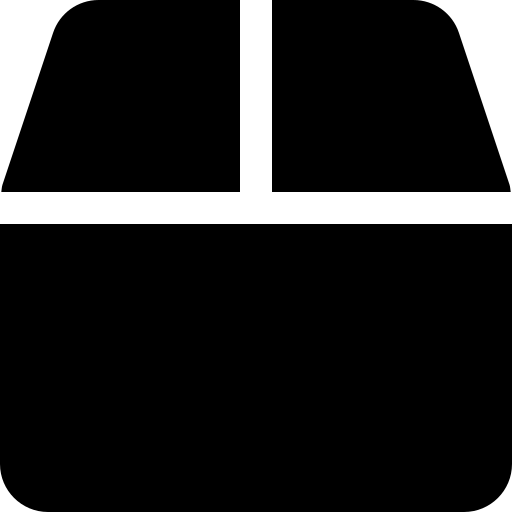
\includegraphics[width=2.5in]{box}%
%\label{fig_first_case}}
%\hfil
%\subfloat[Case II]{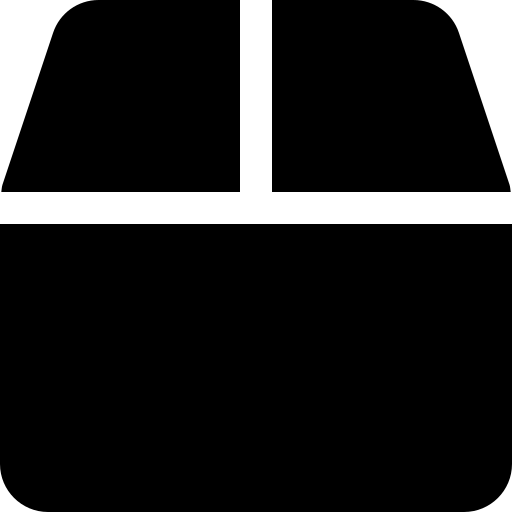
\includegraphics[width=2.5in]{box}%
%\label{fig_second_case}}
%\caption{Simulation results.}
%\label{fig_sim}
%\end{figure*}
%
% Note that often IEEE papers with subfigures do not employ subfigure
% captions (using the optional argument to \subfloat[]), but instead will
% reference/describe all of them (a), (b), etc., within the main caption.


% An example of a floating table. Note that, for IEEE style tables, the 
% \caption command should come BEFORE the table. Table text will default to
% \footnotesize as IEEE normally uses this smaller font for tables.
% The \label must come after \caption as always.
%
%\begin{table}[!t]
%% increase table row spacing, adjust to taste
%\renewcomma\cite{chaum-dc}\cite{chaum-dc}nd{\arraystretch}{1.3}
% if using array.sty, it might be a good idea to tweak the value of
% \extrarowheight as needed to properly center the text within the cells
%\caption{An Example of a Table}
%\label{table_example}
%\centering
%% Some packages, such as MDW tools, offer better commands for making tables
%% than the plain LaTeX2e tabular which is used here.
%\begin{tabular}{|c||c|}
%\hline
%One & Two\\
%\hline
%Three & Four\\
%\hline
%\end{tabular}
%\end{table}


% Note that IEEE does not put floats in the very first column - or typically
% anywhere on the first page for that matter. Also, in-text middle ("here")
% positioning is not used. Most IEEE journals use top floats exclusively.
% However, Computer Society journals sometimes do use bottom floats - bear
% this in mind when choosing appropriate optional arguments for the
% figure/table environments.
% Note that, LaTeX2e, unlike IEEE journals, places footnotes above bottom
% floats. This can be corrected via the \fnbelowfloat command of the
% stfloats package.

\section{Discussion}
Taking all criteria listed above together we get an unexpected set of results. First of all: it seems that unobservable messages is very likely to be asynchronous. It is far harder to hide a multi hop communication if we do not have the possibility to blend into other traffic. Blending into other traffic can be done on a high load node or when collecting up data before sending it on.
\par
We identified clusters of criteria which should not be looked at isolated. These clusters are:

\begin{itemize}
	\item Unidentifiable (pro.1), unknown endpoints (inf.1), no relations between single hops (inf.2), and no direct communication between endpoints (inf.5).
	\item Untrusted infrastructure (inf.3), no central infrastructure (inf.4), and unidentifiable (pro.1).
	\item Reliable(acc.3), and untrusted infrastructure (inf.3) .
\end{itemize}

Looking at the first cluster we see that the users interaction of the system should be equal to the one between nodes. This brings the conclusion that a users node is a specialized message router. Furthermore the infrastructure has to be an established one which has a common legitimate use. This denies the use of a dedicated service. It furthermore leads us to the conclusion, that the chosen service is asynchrnous (or synchronous with message clustering) and allows the service to send and receive messages (e.g. SMTP, or XMMP; but unlike HTTP). 
\par
Since trust is limited to the users any additional measures to hide the message (e.g. such as dummy traffic) have to be user controlled. Sending one big message containing all messages and dummy traffic will result in a big message that decreases in size over time. This is easily detectable. Therefore, the protocol needs a capability to recombine parts of the message without the knowledge of its content.
\par
While using an existing layer of transport we still need to send commonly looking messages. This is only possible by applying techniques of steganography. Unfortunately there are very little elaborated technologies such as F5\cite{f5} are available and there are very good approaches to detect their presence\cite{steganalysisf5}. Even if we hide the message we have to be careful not to run into the dead parrot problem\cite{oakland2013-parrot}.
\par
Looking at the second cluster brings up other conclusions. If we can not trust an infrastructure and the nodes and protocol should be unidentifiable then it means we have to use a common established infrastructure as a transport media. Since no such infrastructure has features mentioned above we need to add them on top of it. As we cannot trust an infrastructure or its admin it means that users must be capable of modifying the behaviour of the infrastructure to match the required results. This has to be done without any privileged access to the server.
\par
The third cluster is not important from a protocol and infrastructure perspective. It is very hard to make a service error prone (acc.3) that includes the possibility to send error messages and react to it considering that we are not able to trust the infrastructure (inf.3). If we cannot trust it we are unable to provide a readable error reply address as it would disclose the senders identity. We do therefore need the possibility to provide a identity or routing token which provides the mean to create a fully unobservable way to reply. Naturally, this does not only apply to the senders identity but to the whole message.
\par
If we have no trust into an infrastructure then we have to establish a kind of discardable identity. If not we do introduce this we do create a kind of pseudonymity enabling an observer to match same identities. Another approach would be that messages are sent to multiple destinations (could be done using a DC algorithm\cite{chaum-dc} or an improved version of it such as\cite{golle:eurocrypt2004}, or Xor-Trees\cite{xor-trees}) without knowing the recipient. It could even be used to recombine multiple messages into one without the knowledge of any node that it has been done.
\par
Another important criteria is "not-abuseable" (acc.4). Having a system which sends unobservable messages makes it easy to blackmail someone. It is therefore vitally important to add unobservable routing information to a message to make sure that a legitimate recipient is capable of identifying the senders identity. Naturally this could be done by a signature. The problem with a signature approach is that as of today we do not have a possibility to find a trustworthy real world identity to a digital identity. We could enforce the use of certificates which contain real world information but by doing so we must trust third party infrastructure (violates inf.3) and add considerable complexity in the use of such a system (may violate acc.1).

\section{Conclusion}
As outlined in the previous sections being unobservable is tricky by itself. The main problem however is to make unobservable messages acceptable for every days use. To achieve this we need to take into account that people are not really aware of the extend being observed. And their readiness to invest efforts into this field is very limited. 
\par
Summing up the findings based on the requirements it looks as follows:
\begin{itemize}
	\item Has to build on one or more established message transmission systems. Criteria are:
	\begin{itemize}
		\item High load or asynchronous behaviour.
		\item Symmetric behaviour in terms of routing.
		\item Usable by steganography.
	\end{itemize} 
	\item Based on well known clients or having a custom one to behave similarly.
	\item Able to recombine message parts to one big message without knowing its content.
	\item Ability to send error messages to the unknown sender.
	\item Ability to modify routing behaviour without modifying the underlying infrastructure.
	\item Ability to hide next hop recipient or sender either by \ldots
	\begin{itemize}
		\item introduce discardable identities
		\item sending to multiple targets without knowing the true recipient.
	\end{itemize}
	\item A routing token which allows to be attached to a message of unknown content. This token hides the recipient and the message from an observer.
\end{itemize}







% if have a single appendix:
%\appendix[Proof of the Zonklar Equations]
% or
%\appendix  % for no appendix heading
% do not use \section anymore after \appendix, only \section*
% is possibly needed

% use appendices with more than one appendix
% then use \section to start each appendix
% you must declare a \section before using any
% \subsection or using \label (\appendices by itself
% starts a section numbered zero.)
%


\appendices
\section{Definitions}\label{app:definitions}
\subsection{Definition of "observer"}
As an observer of the system we assume the following attributes:
\begin{itemize}
	\item Available founding is huge.
	\item Can have own mailer infrastructure.
	\item Is able to read, write or modify network data freely at any point of the net.
\end{itemize}
His intensions are:
\begin{itemize}
	\item Discover message flows
	\item Discover message contents
	\item Identify users of the system
\end{itemize}

\subsection{Definition of "user"}
The assumed user of the system is:
\begin{itemize}
	\item Does care about privacy.
	\item Does or does not have support from a mail server admin.
	\item Has no special computer knowhow.
	\item Has the ability to install a program or plugin on his personal computer.
	\item Has no cryptographic knowhow.
	\item Is using a device with enough calculation power to solve cryptographic tasks.
\end{itemize}
His intensions are:
\begin{itemize}
	\item Send personal or confidential Information securely to another user
\end{itemize}
His expectations are:
\begin{itemize}
	\item System should be easy to configure and maintain (in an ideal world: Zero touch). 
	\item System should be fast.
	\item System should be reliable.
	\item System should work on any client he is using.
	\item System should not be a legal problem to him or any of his peers.
\end{itemize}
\subsubsection{Subclasses of users} 
Users may be split into two groups.
\begin{itemize}
	\item There is always one sender of a message.
	\item There is one or more recipient of a message.
\end{itemize}
There may be certain members of these groups which do not care about privacy may not be using an unobservable system .

\subsection{Definition of "node"}
The assumed node of the system is:
\begin{itemize}
	\item Server publicly reachable.
	\item Server participating in the whole system.
	\item serves one or more defined purposes.
	\item does hove users participating in the unobservable system and other users.
\end{itemize}

\subsection{Definition of "owner"}
The assumed infrastructure owner of the system is:
\begin{itemize}
	\item Does care about privacy.
	\item Has considerable computer knowhow.
	\item Has the ability to install programs or plugins.
	\item Has possibly no cryptographic knowhow.
	\item Does know his own infrastructure.
	\item Is using an Infrastructure with enough calculation power to solve cryptographic tasks.
\end{itemize}
His intensions are:
\begin{itemize}
	\item Support his users in sending personal or confidential information securely to another user
\end{itemize}
His expectations are:
\begin{itemize}
	\item System should be easy to configure and maintain (in an ideal world: Zero touch). 
	\item System should be fast.
	\item System should be reliable.
	\item System should work on any client he is using.
	\item System should not be a legal problem for him or his company.
	\item System should still allow him to do regulatory tasks such as virus scanning or backup.
\end{itemize}

% you can choose not to have a title for an appendix
% if you want by leaving the argument blank

% use section* for acknowledgement
\ifCLASSOPTIONcompsoc
  % The Computer Society usually uses the plural form
  \section*{Acknowledgments}
\else
  % regular IEEE prefers the singular form
  \section*{Acknowledgment}
\fi


The authors would like to thank their families for being so patient with them, Dr. Craig Hamilton and Dr. Manolis Sifalakis for their thoughts on the paper.


% Can use something like this to put references on a page
% by themselves when using endfloat and the captionsoff option.
\ifCLASSOPTIONcaptionsoff
  \newpage
\fi



% trigger a \newpage just before the given reference
% number - used to balance the columns on the last page
% adjust value as needed - may need to be readjusted if
% the document is modified later
%\IEEEtriggeratref{8}
% The "triggered" command can be changed if desired:
%\IEEEtriggercmd{\enlargethispage{-5in}}

% references section

% can use a bibliography generated by BibTeX as a .bbl file
% BibTeX documentation can be easily obtained at:
% http://www.ctan.org/tex-archive/biblio/bibtex/contrib/doc/
% The IEEEtran BibTeX style support page is at:
% http://www.michaelshell.org/tex/ieeetran/bibtex/
\bibliographystyle{IEEEtran}
% argument is your BibTeX string definitions and bibliography database(s)
\bibliography{IEEEabrv,../inc/bib/unclassified/Anonbib/anonbib,../mailvortex}
%\bibliography{IEEEabrv,../bib/paper}
%
% <OR> manually copy in the resultant .bbl file
% set second argument of \begin to the number of references
% (used to reserve space for the reference number labels box)
%\begin{thebibliography}{1}
%
%\bibitem{IEEEhowto:kopka}
%H.~Kopka and P.~W. Daly, \emph{A Guide to {\LaTeX}}, 3rd~ed.\hskip 1em plus
%  0.5em minus 0.4em\relax Harlow, England: Addison-Wesley, 1999.
%
%\end{thebibliography}

% biography section
% 
% If you have an EPS/PDF photo (graphicx package needed) extra braces are
% needed around the contents of the optional argument to biography to prevent
% the LaTeX parser from getting confused when it sees the complicated
% \includegraphics command within an optional argument. (You could create
% your own custom macro containing the \includegraphics command to make things
% simpler here.)
%\begin{IEEEbiography}[{\includegraphics[width=1in,height=1.25in,clip,keepaspectratio]{mshell}}]{Michael Shell}
% or if you just want to reserve a space for a photo:
\ifCLASSOPTIONpeerreview
\else
\vfill
\begin{IEEEbiography}[{\includegraphics[width=1in,height=1.25in,clip,keepaspectratio]{../inc/biography/passphoto}}]{Martin Gwerder}
% !TeX spellcheck = en_GB

Martin Gwerder was born 20. July 1972 in Glarus, Switzerland. He is currently a doctoral Student at the University of Basel. After having concluded his studies at the polytechnic at Brugg in 1997, he did a postgraduate study as a master of business and engineering. Following that, he changed to the university track doing an MSc in Informatics at FernUniversit\"at in Hagen. While doing this he constantly broadened his horizon by working for industry, banking and government as  engineer and architect in security related positions. He currently holds a lecturer position for cloud and security at the University of Applied Sciences Northwestern Switzerland. His main expertise lays in the field of networking related problems dealing with data protection, distribution, confidentiality and anonymity.
\end{IEEEbiography}
\fi

% if you will not have a photo at all:
%\begin{IEEEbiographynophoto}{John Doe}
%Biography text here.
%\end{IEEEbiographynophoto}

% insert where needed to balance the two columns on the last page with
% biographies
%\newpage

%\begin{IEEEbiographynophoto}{Jane Doe}
%Biography text here.
%\end{IEEEbiographynophoto}

% You can push biographies down or up by placing
% a \vfill before or after them. The appropriate
% use of \vfill depends on what kind of text is
% on the last page and whether or not the columns
% are being equalized.

%\vfill

% Can be used to pull up biographies so that the bottom of the last one
% is flush with the other column.
%\enlargethispage{-5in}



% that's all folks
\end{document}


